% !TeX root = main.tex
% !TEX program = pdflatex

\chapter{Sensores Ópticos}\label{cap:opticos}

Los sensores ópticos convierten la energía radiante (fotones) en señales eléctricas. En este capítulo analizaremos los dispositivos basados en semiconductores que operan mediante la interacción de la luz con la materia, abarcando desde detectores puntuales como fotodiodos y fototransistores hasta sensores de imagen matriciales como los sistemas CCD y CMOS.

\section{Fundamentos de la Detección Óptica}\label{sec:fundamentos_opticos}

La detección óptica es una aplicación tecnológica directa de los principios de la \emph{física cuántica}. Se fundamenta en el \emph{efecto fotoeléctrico interno}, un proceso donde la luz interactúa con la materia a nivel atómico. Este fenómeno demostró definitivamente la naturaleza dual de la luz: los fotones actúan como paquetes discretos de energía, una idea tan revolucionaria que permitió a Albert Einstein recibir el Premio Nobel de Física en 1921 por su explicación teórica.

\marginnote{\textbf{Einstein y el Nobel:} Aunque es mundialmente famoso por la Relatividad, el comité del Nobel le otorgó el premio específicamente por descubrir la ley del efecto fotoeléctrico, sentando las bases de la mecánica cuántica al tratar la luz como un flujo de partículas (fotones).}

A diferencia del efecto fotoeléctrico externo (donde los electrones son arrancados de la superficie de un metal), en el \emph{efecto interno} los portadores permanecen dentro del semiconductor pero cambian su estado energético. Cuando un fotón incide sobre el cristal, si su energía ($E = h \cdot f$) es superior a la energía de banda prohibida (\textit{bandgap}, $E_g$), un electrón de la banda de valencia absorbe esa energía y promociona a la banda de conducción.

\paragraph{Bandas de Energía en Semiconductores}
En un semiconductor, los electrones se organizan en niveles agrupados en bandas de energía. Existen dos bandas principales: la \emph{banda de valencia} y la \emph{banda de conducción}. Es crucial entender que la \emph{banda de conducción posee mayor energía} que la \emph{banda de valencia}. La banda de conducción se encuentra por encima de la banda de valencia. Los electrones tienden naturalmente a ocupar los estados de mínima energía, por lo que permanecen atrapados en la \emph{banda de valencia} (ligados a los átomos). 

\marginnote{\textbf{La analogía del estante:} Imagina un balón en el suelo (valencia) y un estante elevado (conducción). El balón no subirá solo porque el estante es un estado de mayor energía potencial. Para "promocionarlo", necesitas darle un impulso (el fotón) con energía suficiente para superar la altura del estante.}

Por encima de la banda de valencia se sitúa la \emph{banda de conducción}, que representa el nivel energético necesario para que las cargas se muevan libremente. Para que un electrón realice este salto entre bandas hacia un estado más energético, debe absorber energía externa. La región que separa ambos niveles es el \emph{bandgap} ($E_g$): una barrera que el electrón solo puede vencer si un fotón le entrega exactamente la energía que le falta para llegar arriba.

\begin{marginfigure}
    \centering
    \shorthandoff{>}
    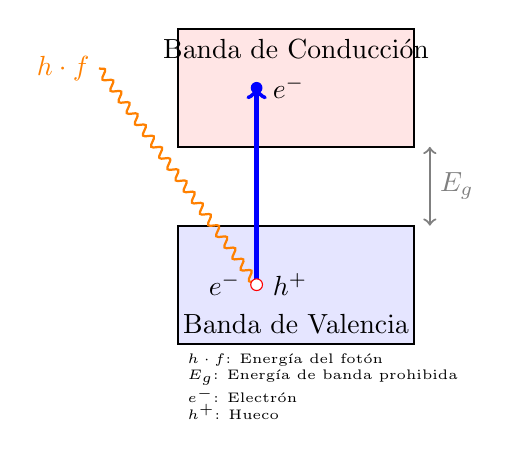
\begin{tikzpicture}[scale=1]
        % Bandas de energía
        \draw[thick, fill=blue!10] (0,0) rectangle (3,1.5);
        \node at (1.5, .25) {Banda de Valencia};
        
        \draw[thick, fill=red!10] (0,2.5) rectangle (3,4);
        \node at (1.5, 3.75) {Banda de Conducción};
        
        % Bandgap
        \draw[<->, thick, gray] (3.2, 1.5) -- (3.2, 2.5) node[midway, right] {$E_g$};
        
        % Electrón en banda de valencia
        \node[circle, fill=blue, inner sep=1.5pt, label=left:{$e^-$}] (electron) at (1, 0.75) {};
        
        % Fotón incidente
        \draw[orange, thick, decoration={snake, amplitude=1.5pt, segment length=5pt}, decorate] (-1, 3.5) -- (electron.center);
        \node[orange, left] at (-1, 3.5) {$h \cdot f$};
        
        % Flecha de promoción del electrón
        \draw[->, ultra thick, blue] (electron.center) -- (1, 3.25) node[midway, right, black] {};
        
        % Electrón en banda de conducción
        \node[circle, fill=blue, inner sep=1.5pt, label=right:{$e^-$}] (electron_cond) at (1, 3.25) {};
        
        % Hueco en banda de valencia
        \node[circle, draw=red, fill=white, inner sep=1.5pt, label=right:{$h^+$}] (hole) at (1, 0.75) {};
        
        % Leyenda
        \node[align=left, font=\tiny, anchor=north west] at (0, -0) {
            $h \cdot f$: Energía del fotón \\
            $E_g$: Energía de banda prohibida \\
            $e^-$: Electrón \\
            $h^+$: Hueco
        };
    \end{tikzpicture}
    \caption[Efecto fotoeléctrico interno.]{Representación esquemática del efecto fotoeléctrico interno. Un fotón con energía suficiente ($h \cdot f > E_g$) excita un electrón de la banda de valencia a la banda de conducción, generando un par electrón-hueco. La \emph{banda de valencia} contiene los electrones ligados a los átomos, mientras que la \emph{banda de conducción} contiene los electrones libres que pueden conducir electricidad.}\label{fig:efecto_fotoelectrico_interno}
\end{marginfigure}

Este salto energético genera un \emph{par electrón-hueco}, transformando instantáneamente un estímulo óptico en portadores de carga eléctrica móviles. La importancia de este descubrimiento es incalculable: es el eslabón fundamental que permite convertir la luz en información, siendo la base de la imagen digital, las comunicaciones por fibra óptica y la energía solar fotovoltaica.

\paragraph{Respuesta Espectral}
La sensibilidad de un sensor óptico no es constante para todas las longitudes de onda. Se define mediante la \emph{responsividad} ($R$), que relaciona la corriente generada con la potencia óptica incidente (\unit{A/W}). Como se muestra en la Figura~\ref{fig:curva_espectral}, los sensores de Silicio (Si) son ideales para el espectro visible e infrarrojo cercano, mientras que el Arseniuro de Galio-Indio (InGaAs) se emplea en comunicaciones por fibra óptica.

\marginnote{\textbf{Uso de Silicio en el Espectro Visible?} El silicio se usa en el espectro visible a pesar de que el pico de responsividad del silicio está en el infrarrojo ($\approx \qty{900}{nm}$). El silicio se utiliza masivamente en el visible por: 
1. \emph{Sensibilidad:} Sigue siendo suficiente en el rango \qtyrange{400}{700}{nm}.
2. \emph{Coste/Integración:} Es el material base de la industria microelectrónica (CMOS).
3. \emph{Filtros IR:} Se emplean filtros de corte (\textit{IR-cut filters}) para bloquear el pico infrarrojo y ajustar la respuesta a la del ojo humano.}

\begin{marginfigure}
    \centering
    \shorthandoff{>}
    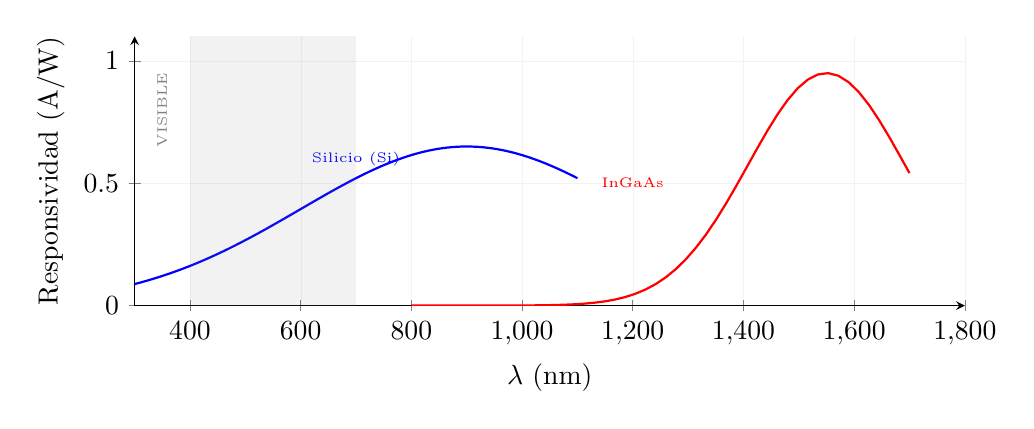
\begin{tikzpicture}
        \begin{axis}[
            width=\linewidth, height=5cm,
            xlabel={$\lambda$ (\qty{}{nm})}, ylabel={Responsividad (A/W)},
            xmin=300, xmax=1800, ymin=0, ymax=1.1,
            axis lines=left, grid=both,
            grid style={line width=.1pt, draw=gray!10},
            legend style={at={(0.95,0.95)}, anchor=north east, draw=none}
        ]
            % Silicio
            \addplot[thick, blue, domain=300:1100, samples=100] {0.65 * exp(-(x-900)^2/180000)};
            \node[blue, font=\tiny] at (axis cs:700, 0.6) {Silicio (Si)};
            
            % InGaAs
            \addplot[thick, red, domain=800:1700, samples=50] {0.95 * exp(-(x-1550)^2/40000)};
            \node[red, font=\tiny] at (axis cs:1200, 0.5) {InGaAs};
            
            % Banda visible sutil
            \fill[gray, opacity=0.1] (axis cs:400,0) rectangle (axis cs:700,1.1);
            \node[gray, rotate=90, font=\tiny] at (axis cs:350, 0.8) {VISIBLE};
        \end{axis}
    \end{tikzpicture}
    \caption[Curvas de responsividad espectral.]{Curvas de responsividad espectral para diferentes materiales. El límite de corte superior viene determinado por el \textit{bandgap} del material.}\label{fig:curva_espectral}
\end{marginfigure}

\marginnote{\textbf{Energía del fotón:} La longitud de onda de corte ($\lambda_c$) es la máxima que puede detectar un sensor:
    \[ \lambda_c \approx \frac{1240}{E_g \text{ (eV)}} \text{ nm} \]
    Para el Silicio ($E_g = \qty{1.12}{eV}$), el corte ocurre cerca de los \qty{1100}{nm}.
}

\section{Fotodiodos}\label{sec:fotodiodos}

Un fotodiodo es una unión PN semiconductora diseñada para operar bajo la incidencia de radiación lumínica. Aunque comparte la estructura física básica con una célula solar, su diseño está optimizado para maximizar la \emph{linealidad} (relación corriente-iluminancia) y la \emph{velocidad de respuesta} (ancho de banda), sacrificando la capacidad de entregar potencia eléctrica a una carga.

\paragraph{Modos de Operación}
El funcionamiento se basa en la generación de portadores de carga mediante la absorción de fotones. Como se ilustra en la Figura~\ref{fig:estructura_fotodiodo}, cuando un fotón con energía $h\nu \geq E_g$ impacta en el dispositivo, crea un par electrón-hueco. La separación de estos portadores por el campo eléctrico de la unión genera una corriente fotogenerada ($I_{ph}$) que es proporcional a la intensidad luminosa.

\begin{marginfigure}
    \centering
    \shorthandoff{>}
    \begin{tikzpicture}[scale=1, >=stealth]
        % --- Cuerpo del semiconductor ---
        % Capa P
        \fill[red!15] (0,1.5) rectangle (5,2.5);
        \node at (3.5,2.15) {Material Tipo P};
        
        % Zona de Deplexión (Región activa)
        \fill[gray!10] (0,1) rectangle (5,1.5);
        \draw[dashed, gray] (0,1.5) -- (5,1.5);
        \draw[dashed, gray] (0,1) -- (5,1);
        \node[gray!70!black] at (3.2,1.25) {Zona de Deplexión};
        
        % Capa N
        \fill[blue!15] (0,0) rectangle (5,1);
        \node at (1.5,0.35) {Material Tipo N};

        % --- Campo Eléctrico Interno ---
        \draw[->, thick, gray!80] (4.7, 1.4) -- (4.7, 1.1) node[midway, right] {$\vec{E}$};

        % --- Fotones ---
        \foreach \x/\yend in {0.6/1.7, 1.3/0.8, 2.0/1.4, 2.7/1.2} {
            \draw[orange, thick, ->, decoration={snake, amplitude=1pt, segment length=5pt}, decorate] 
                (\x, 3.2) -- (\x, \yend);
        }
        \node[orange, font=\bfseries] at (2, 3.4) {$h\nu$ (Fotones)};

        % --- Generación de pares ---
        % Hueco (+) moviéndose hacia P
        \node[circle, fill=red, inner sep=0.5pt, text=white] (h1) at (1.5, 1.3) {\tiny $+$};
        \draw[->, red] (h1.north) -- ++(0, 0.4);
        
        % Electrón (-) moviéndose hacia N
        \node[circle, fill=blue, inner sep=0.5pt, text=white] (e1) at (1.7, 1.2) {\tiny $-$};
        \draw[->, blue] (e1.south) -- ++(0, -0.4);

        % --- Terminales ---
        \draw (2.5, 2.5) -- (2.5, 2.8) node[ocirc] {} node[right] {Ánodo};
        \draw (2.5, 0) -- (2.5, -0.3) node[ocirc] {} node[right] {Cátodo};
        
    \end{tikzpicture}
    \caption[Estructura física de un fotodiodo.]{Estructura interna de un fotodiodo. El campo eléctrico $\vec{E}$ en la zona de deplexión separa rápidamente los pares electrón-hueco generados por la luz, dando lugar a la fotocorriente $I_{ph}$.}\label{fig:estructura_fotodiodo}
\end{marginfigure}

Si este par se genera dentro de la \emph{zona de deplexión}, el intenso campo eléctrico interno $\vec{E}$ separa los portadores antes de que puedan recombinarse: los huecos son arrastrados hacia el ánodo (P) y los electrones hacia el cátodo (N). Este flujo de carga constituye la \emph{fotocorriente} ($I_{ph}$), que circula en sentido inverso (del cátodo al ánodo).

\marginnote{\textbf{Corriente de Oscuridad ($I_d$):} Es la pequeña corriente que fluye por el fotodiodo en ausencia total de luz. Se debe a la generación térmica de portadores y representa el ruido de fondo que limita la resolución del sensor.
}

\paragraph{Linealidad y Responsividad}
La característica más valorada del fotodiodo en instrumentación es su linealidad. La corriente generada es estrictamente proporcional al número de fotones incidentes (flujo radiante $\Phi_e$) sobre una amplia gama de intensidades (hasta 6 o 7 décadas):
\begin{equation}\label{eq:responsividad}
    I_{ph} = \mathcal{R} \cdot \Phi_e
\end{equation}
donde $\mathcal{R}$ es la \emph{responsividad} del dispositivo, expresada en \qty{}{A/W}. 

\marginnote{\textbf{Diferencia con Célula Solar:} Mientras que la célula solar busca maximizar el producto $V \cdot I$ para generar potencia, el fotodiodo se utiliza con \emph{polarización nula o inversa} para garantizar que el tiempo de tránsito de los portadores sea mínimo, permitiendo anchos de banda de varios \qty{}{GHz}.
}

El ingeniero de instrumentación debe elegir entre dos modos de polarización, cada uno con ventajas específicas:

\begin{enumerate}
    \item \emph{Modo Fotovoltaico (Polarización cero)}: El fotodiodo se conecta a un amplificador de transimpedancia con tensión nula. Presenta el menor \emph{ruido de oscuridad} pero es más lento debido a la alta capacidad de unión.
    \item \emph{Modo Fotoconductivo (Polarización inversa)}: Se aplica una tensión inversa ($V_R$). Esto ensancha la zona de deplexión, reduciendo la capacidad de unión y aumentando drásticamente la \emph{velocidad de respuesta}. Sin embargo, aparece una corriente de oscuridad que limita la sensibilidad.
\end{enumerate}

La elección del modo de trabajo determina el punto de operación sobre la curva característica del semiconductor. Como se ilustra en la Figura~\ref{fig:curva_vi_modos}, la luz desplaza la curva del diodo hacia valores de corriente negativa (fotocorriente).

\begin{marginfigure}
    \centering
    \shorthandoff{>}
    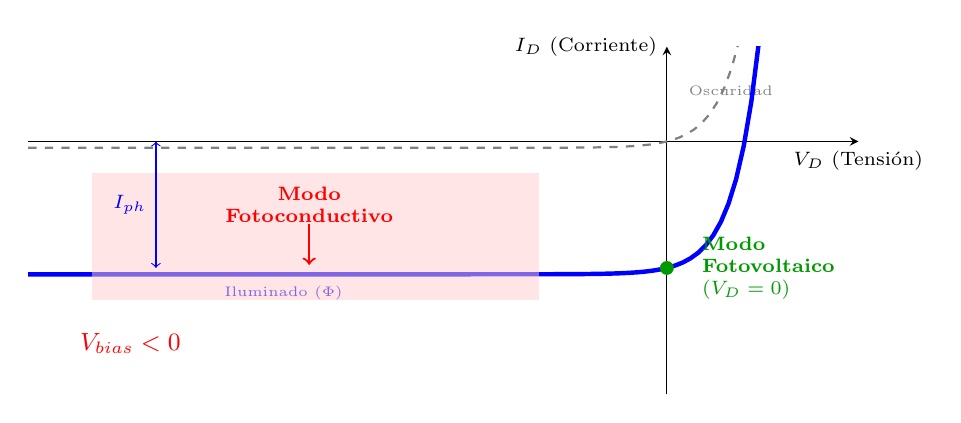
\begin{tikzpicture}
        \begin{axis}[
            width=\linewidth, height=6cm,
            xlabel={$V_D$ (Tensión)}, ylabel={$I_D$ (Corriente)},
            xmin=-5, xmax=1.5, ymin=-4, ymax=1.5,
            axis lines=center,
            xtick={0}, ytick={0},
            font=\scriptsize,
            xlabel style={at={(ticklabel* cs:1)}, anchor=north},
            ylabel style={at={(ticklabel* cs:1)}, anchor=east},
        ]
            % Curva en oscuridad (Diodo normal)
            \addplot[thick, gray, dashed, domain=-5:0.8, samples=100] {0.1*(exp(x/0.2)-1)};
            \node[gray, font=\tiny] at (axis cs:0.5, 0.8) {Oscuridad};

            % Curva con Iluminación (Iph = 2)
            \addplot[ultra thick, blue, domain=-5:0.9, samples=100] {0.1*(exp(x/0.2)-1) - 2};
            \node[blue, font=\tiny] at (axis cs:-3, -2.4) {Iluminado ($\Phi$)};

            % --- MODO FOTOCONDUCTIVO ---
            \fill[red!20, opacity=0.5] (axis cs:-4.5,-2.5) rectangle (axis cs:-1,-0.5);
            \node[red, align=center] at (axis cs:-2.8, -1) {\textbf{Modo}\\\textbf{Fotoconductivo}};
            \draw[red, thick, ->] (axis cs:-2.8, -1.3) -- (axis cs:-2.8, -1.95);
            \node[red, font=\small] at (axis cs:-4.2, -3.2) {$V_{bias} < 0$};

            % --- MODO FOTOVOLTAICO ---
            \fill[green!60!black] (axis cs:0,-2) circle (2.5pt);
            \node[green!60!black, anchor=west, align=left] at (axis cs:0.2, -2) {\textbf{Modo}\\\textbf{Fotovoltaico}\\($V_D = 0$)};
            
            % Flecha de Iph
            \draw[<->, blue] (axis cs:-4, 0) -- (axis cs:-4, -2) node[midway, left] {$I_{ph}$};

        \end{axis}
    \end{tikzpicture}
    \caption[Modos de operación en la curva V-I.]{Curva característica del fotodiodo. El \emph{Modo Fotovoltaico} opera en el origen de tensiones ($V_D=0$), anulando la corriente de oscuridad. El \emph{Modo Fotoconductivo} opera con polarización inversa, aumentando la velocidad de respuesta.}\label{fig:curva_vi_modos}
\end{marginfigure}

\paragraph{Física del Modo Fotoconductivo}
Al aplicar una tensión de polarización inversa ($V_{bias} < 0$), los portadores mayoritarios son alejados de la unión, lo que ensancha la zona de deplexión ($w$). Puesto que un fotodiodo se comporta eléctricamente como un condensador de placas paralelas, su capacidad de unión ($C_j$) se reduce según la expresión:
\begin{equation}\label{eq:capacidad_union}
    C_j = \frac{\epsilon A}{w} \propto \frac{1}{\sqrt{V_{bi} + |V_{bias}|}}
\end{equation}
donde $V_{bi}$ es la tensión de barrera interna. Esta reducción de capacidad es fundamental en instrumentación de alta velocidad, ya que disminuye el tiempo de subida del sensor ($t_r \approx 2,2 \cdot R_L C_j$), permitiendo anchos de banda de megahercios a gigahercios.

\paragraph{Física del Modo Fotovoltaico}
En este modo, el ánodo y el cátodo se mantienen al mismo potencial, normalmente mediante la tierra virtual de un amplificador de transimpedancia. Al no existir un campo eléctrico externo, no hay una corriente de deriva térmica significativa. La Figura~\ref{fig:tia_pd} muestra que la corriente de oscuridad se anula, ya que el punto de operación se encuentra en el origen de tensiones ($V_D = 0$).

\marginnote{\textbf{Linealidad Precisa:} El modo fotovoltaico es el más lineal. Al operar con $V_D = 0$, evitamos que la resistencia serie del dispositivo y las variaciones de la corriente de saturación afecten a la medida, obteniendo una relación corriente-luz casi perfecta.
}

Como consecuencia, la \emph{corriente de oscuridad} ($I_{dark}$) se reduce al mínimo teórico, eliminando el principal componente de ruido sistemático. Esta configuración es obligatoria cuando se pretenden medir flujos luminosos extremadamente bajos, donde cualquier fuga térmica enmascararía la señal generada por los fotones.


El amplificador de transimpedancia TIA es el componente principal de un fotodiodo operado en modo fotovoltaico. Su función principal es convertir una corriente de entrada en una tensión de salida. Dado que un fotodiodo se comporta esencialmente como una fuente de corriente proporcional a la luz, y que la mayoría de los sistemas de adquisición (ADC) requieren una entrada de tensión, es necesario un bloque convertidor corriente-tensión ($I \to V$). El circuito estándar para esta tarea es el \emph{Amplificador de Transimpedancia}. El nombre proviene de la Ley de Ohm ($V=I \cdot Z$). Como la ganancia del circuito relaciona una tensión de salida con una corriente de entrada, las unidades de dicha ganancia son Ohmios (\unit{ohms}).

\begin{equation}
G = \frac{V_{out}}{I_{in}} \implies [\text{V}/{\text{A}}] = [\Omega]
\end{equation}
Por tanto, la ganancia es una "impedancia de transferencia" o transimpedancia.


Aquí tienes la explicación técnica detallada para incluir en tus apuntes, justificando por qué es el compañero inseparable del fotodiodo:

\marginnote{\textbf{Resumen para el diseño:} 
    \begin{itemize}
        \item \emph{¿Velocidad?} $\rightarrow$ Fotoconductivo ($V_{bias} < 0$).
        \item \emph{¿Bajo Ruido?} $\rightarrow$ Fotovoltaico ($V_{bias} = 0$).
    \end{itemize}
}


\begin{marginfigure}
    \centering
    \shorthandoff{>}
    \begin{tikzpicture}[american, scale=1]
        \ctikzset{amplifiers/fill=blue!5, capacitors/scale=0.6}
        % Op amp
        \draw (2,1) node[op amp] (oa) {};
        % Fotodiodo
        \draw (oa.-) -- ++(-1,0) coordinate(nodePD) to[photodiode, l=$I_{ph}$, *-] ++(0,-1.5) node[ground](GND){};
        % Realimentación
        \draw (oa.-) -- ++(0,1) coordinate(FB) to[R, l=$R_f$] (FB -| oa.out) -- (oa.out) node[circ]{};
        \draw (oa.+) -- (oa.+ |- GND) node[ground]{};
        % Salida
        \draw (oa.out) to[short, -o] ++(0.5,0) node[right] {$V_{out} = -I_{ph}R_f$};
        
        \node[red, font=\tiny, align=center] at (0.5, 0.5) {Tierra\\Virtual};
    \end{tikzpicture}
    \caption[Amplificador de transimpedancia para fotodiodo.]{Acondicionamiento típico de un fotodiodo (\emph{Transimpendance Ampifier}, TIA). El operacional mantiene el diodo en modo fotovoltaico (tensión nula) para maximizar la linealidad.}\label{fig:tia_pd}
\end{marginfigure}

\marginnote{
    \textbf{Fotodiodo PIN:} 
    Muchos sensores modernos introducen una capa intrínseca (I) entre la P y la N. Esto permite captar más fotones y reducir aún más la capacidad, logrando anchos de banda de \qty{}{GHz}.
}



\section{Fototransistores}\label{sec:fototransistores}

Un fototransistor combina un fotodiodo y un amplificador bipolar en el mismo cristal. La luz incide sobre la unión colector-base, generando una corriente que actúa como corriente de base ($I_b$).

\begin{equation}
    I_c = \beta \cdot I_{ph}
\end{equation}

Como se muestra en la Figura~\ref{fig:fototransistor}, el dispositivo ofrece una \textbf{ganancia intrínseca} ($\beta$), lo que simplifica el circuito de acondicionamiento al no requerir etapas de amplificación externas complejas. Sin embargo, su tiempo de respuesta es mucho mayor que el de un fotodiodo (µs frente a ns).

\begin{marginfigure}[2em]
    \centering
    \shorthandoff{>}
    \begin{tikzpicture}[american, scale=1]
        % Símbolo fototransistor
        \draw (0,0) node[npn, photo] (pt) {};
        \draw (pt.C) -- ++(0,0.5) to[R, l=$R_c$] ++(0,1.5) node[above] {$V_{CC}$};
        \draw (pt.E) node[ground]{};
        \draw (pt.C) to[short, *-o] ++(1,0) node[right] {$V_{out}$};
        
        \node[orange] at (-1, 0.5) {$h\nu$};
    \end{tikzpicture}
    \caption[Configuración de fototransistor.]{Fototransistor en configuración de emisor común. La ganancia $\beta$ proporciona una señal de salida robusta a cambio de una menor velocidad de conmutación.}\label{fig:fototransistor}
\end{marginfigure}

\section{Sensores de Imagen: CCD y CMOS}\label{sec:sensores_imagen}

Los sensores de imagen son matrices de millones de fotodetectores (píxeles). Aunque ambos se basan en el silicio, su arquitectura de lectura es radicalmente distinta.

\paragraph{CCD (\textit{Charge-Coupled Device})}
Los píxeles actúan como pozos de potencial que acumulan carga. La lectura es analógica y secuencial: las cargas se "desplazan" de un píxel a otro como en una brigada de cubos de agua hasta un único amplificador de salida. 
\begin{itemize}
    \item \textbf{Ventaja}: Alta uniformidad y bajo ruido.
    \item \textbf{Desventaja}: Alto consumo y lectura lenta.
\end{itemize}

\paragraph{CMOS (\textit{Complementary Metal-Oxide-Semiconductor})}
Cada píxel posee su propio amplificador y conversor A/D (\textit{Active Pixel Sensor}). La lectura es digital y paralela, similar a una memoria RAM.
\begin{itemize}
    \item \textbf{Ventaja}: Integración de funciones (Smart Sensors), bajo coste y alta velocidad.
    \item \textbf{Desventaja}: Mayor ruido de patrón fijo (\textit{Fixed Pattern Noise}).
\end{itemize}

\begin{table}[ht]
    \centering
    \small
    \caption{Comparativa técnica de sensores ópticos para instrumentación.}\label{tab:comparativa_optica}
    \begin{tabularx}{\linewidth}{l X X X}
        \toprule
        \textbf{Parámetro} & \textbf{Fotodiodo} & \textbf{Fototransistor} & \textbf{LDR} \\
        \midrule
        Linealidad & Excelente & Regular & Pobre (log) \\
        Velocidad & Muy alta (\unit{ns}) & Media (\unit{\mu s}) & Muy baja (\unit{ms}) \\
        Sensibilidad & Baja (\unit{nA/lux}) & Alta (\unit{mA/lux}) & Variable \\
        Acondic. & Crítico (TIA) & Sencillo & Divisor tensión \\
        \bottomrule
    \end{tabularx}
\end{table}

\marginnote{\textbf{Ruido de Disparo (\textit{Shot Noise}):} Es el ruido dominante en sensores ópticos. Se debe a la naturaleza discreta de los fotones y electrones. Su valor eficaz es $I_n = \sqrt{2qI\Delta f}$.
}

\cleardoublepage